\begin{solution}{Question 4(c)}\label{ques:4c}
    \begin{question}
      Implement $H()$ and $H_r()$ in Python/Java for $M = 10^4$ and the following different choices of sets of size $n = 100$: For $k \in [1, n]$, $S_k$ is union of $\{0, n, 2n, 3n, \ldots, (k-1)n\}$ and $n-k$ random elements in $U$.\\
Obtain a plot of Max-chain-length for hash functions $H()$, $H_r()$ over different choices of sets $S_k$ defined above. Note that you must choose a different random $r$ for each choice of $S_k$. Provide a justification for your plots.
    \end{question}
    \tcblower{}
    \begin{proof}[Solution]
      We observe that the maximum chain length increases almost linearly for $H()$ while it remains approximately constant for $H_R()$. This is because as $k$ increases, the set $S_K$ becomes less and less random. $H(x) = 0$ for $x = i\cdot n$ and this is what amounts to the maximum chain length as $k$ increases. However, in the case of $H_r()$, the set $S_k$ is transformed to a random set and therefore the maximum chain length remains constant with an exepctation of $2$.
      \begin{figure}[H]
        \centering
        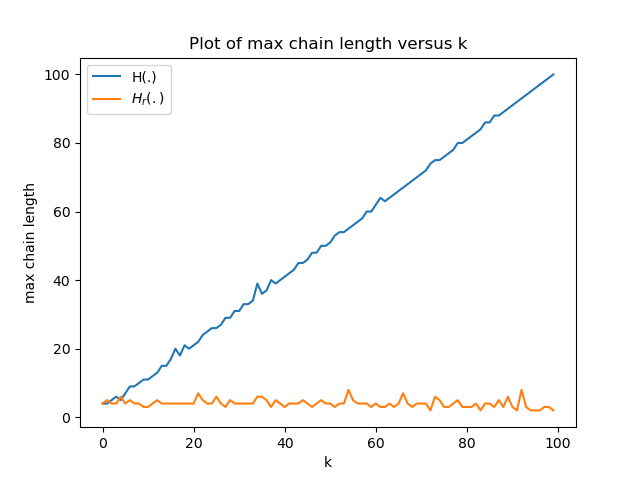
\includegraphics[width=0.5\linewidth]{4c.png}
        \caption{Plot}
      \end{figure}
    \end{proof}
\end{solution}
